%!TEX TS-program = xelatex
\documentclass[]{friggeri-cv}
\usepackage{afterpage}
\usepackage{hyperref}
\usepackage{color}
\usepackage{xcolor}
\hypersetup{
    pdftitle={},
    pdfauthor={},
    pdfsubject={},
    pdfkeywords={},
    colorlinks=false,       % no lik border color
   allbordercolors=white    % white border color for all
}
%\addbibresource{bibliography.bib}
\RequirePackage{xcolor}
\definecolor{pblue}{HTML}{0395DE}

\begin{document}
%% CV language selection: Spanish(ES), English(EN). 
\newtoggle{ES}
\newtoggle{EN}
\toggletrue{EN}
\togglefalse{ES}

%% CV professional profiles: project coordination (CO), systems engineer(SYS) or software engineer (SOFT)
\newtoggle{CO}
\newtoggle{SYS}
\newtoggle{SOFT}
\togglefalse{CO}
\togglefalse{SYS}
\toggletrue{SOFT}

%% Add candidate picture to cv
\newtoggle{picture}
\toggletrue{picture}
%\togglefalse{picture}

\header{Pablo}{Miangolarra}
{\iftoggle{ES}{Ingeniero software}{}
\iftoggle{EN}{Software engineer}{}}
\newline
\newline 
\newline
\newline 
% Fake text to add separator      
\fcolorbox{white}{gray}{\parbox{\dimexpr\textwidth-2\fboxsep-2\fboxrule}{%
.....
}}

% In the aside, each new line forces a line break
\begin{aside}
% Personal picture
\iftoggle{picture}{
\includegraphics[width=3.5cm]{img/cv_picture}}{\vspace{5cm}}
\iftoggle{ES}{\section{Dirección}}{} 
\iftoggle{EN}{\section{Address}}{}
Calle valle de Boi, 8
28054 Madrid
    ~
\iftoggle{ES}{\section{Tfno. \& Skype}}{} 
\iftoggle{EN}{\section{Phone \& Skype}}{}
    +34 665 111 427
    pablo.miangolarra
    ~
\section{E-Mail}
    \href{mailto:pablo.miangolarra@gmail.com}{\textbf{pablo.miangolarra@}\\gmail.com}
    ~
\section{Blog \& web}
    \href{https://fidgetyfig.wordpress.com}{fidgetyfig.wordpress.com}
    \href{https://twitter.com/miangolarra}{twitter.com/miangolarra}
    ~
    %\color{blue} \rule{\linewidth}{1mm}
    %\textbf{Destacado para el puesto}
    % OR
    \vspace{1cm}
    ~
    ~
    ~
    ~
    
\includegraphics[width=3cm]{img/logo_iese}
%\section{Programming}
%    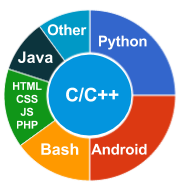
\includegraphics[scale=0.62]{img/programming.png}
%    ~
%  \section{OS Preference}
   % \textbf{GNU/Linux}
\includegraphics[scale=0.40]{img/5stars.png}
    %\textbf{Unix}
\includegraphics[scale=0.40]{img/4stars.png}
    %\textbf{MacOS}
\includegraphics[scale=0.40]{img/2stars.png}
    %\textbf{Windows}
\includegraphics[scale=0.40]{img/1stars.png}
    %~
  %\section{Personal Skills}
    %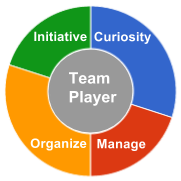
\includegraphics[scale=0.62]{img/personal.png}
   % ~
\end{aside}


%% Project: cv
%% Author: Pablo Miangolarra
%% Last update: 21 November 2016
%%
\iftoggle{ES}{\section{Educación}}{}
\iftoggle{EN}{\section{Education}}{}
\label{sec:education}
\begin{entrylist}
\iftoggle{ES}{
  \entry
    {08/14 - 12/16}
    {European Master in Software Engineering}
    {TU Kaiserslautern, Alemania}
    {%A la espera de nota final.
    %\color{blue} \rule{\linewidth}{1mm} 
    Asignaturas: gestión de proyectos software, metodologías ágiles, ingeniería de requisitos, ingeniería en linea de producción, arquitectura software, calidad del software, diseño interactivo, interacción humano máquina, interfaces de usuario inteligentes, métricas software y metodologías de investigación.
    \emph{Título de proyecto final: "Diseño colaborativo de aplicaciones móviles".}\\
    %\color{blue} \rule{\linewidth}{1mm} 	
    }
}{}
\iftoggle{EN}{
  \entry
    {08/14 - 12/16}
    {Master in Software Engineering}
    {TU Kaiserslautern, Germany}
    {%A la espera de nota final.
    %\color{blue} \rule{\linewidth}{1mm} 
    Courses: Software project management, agile methodologies, requirements engineering, product line engineering, software architecture, software quality, interactive design, human-computer interaction, intelligent user interfaces, software metrics and research methodologies.\\
    \emph{Master thesis's title: "Mobile application collaborative design".}\\
    %\color{blue} \rule{\linewidth}{1mm} 	
    }
}{}
\iftoggle{ES}{
  \entry
    {03/10 - 02/12}
    {Ingeniería superior en informática}
    {Universidad Rey Juan Carlos, España}
    {Especialización en sistemas informáticos, nota media: 7,7/10.\\
    Asignaturas: ingeniería del software, seguridad del software, sistemas telemáticos y aplicaciones para la web: html, css, JavaScript, xml, xslt, php, python, django.\\
    \emph{Título de proyecto final:  "Sistema distribuido para la gestión de sensores heterogéneos en instalaciones críticas".}\\}
}{}
\iftoggle{EN}{
  \entry
    {03/10 - 02/12}
    {Senior engineering in Computer Sciences}
    {Rey Juan Carlos University, Spain}
    {Specialisation in information systems, average score: 7,7/10.\\
    Courses: Software engineering, software security, telematic systems and web applications: html, css, javascript, xml, xslt, php, python, django.\\
    \emph{Master thesis's title:  "Distributed system for the management of heterogeneous sensors in critical infrastructures".}\\}
}{}
\iftoggle{ES}{
   \entry
    {09/05 - 02/10}
    {Ingeniería técnica en informática}
    {Universidad Rey Juan Carlos, España}
    {Especialización en robótica, nota media: 7,37/10\\
    Asignaturas: visión computacional, sistemas operativos, redes y programación: Java, Shell, JavaRMI, C, C++, PL/SQL, OpenCV, OpenGL, VHDL.\\
    Tercero de carrera cursado en la Universidad de Lancaster, Inglaterra.\\
    \emph{Título de proyecto final:  "Memoria visual 3D para robot móvil con par estéreo".}}
}{}
\iftoggle{EN}{
   \entry
    {09/05 - 02/10}
    {Bachelor in Computer Sciences}
    {Rey Juan Carlos University, Spain}
    {Specialisation in robotics, average score: 7,37/10\\
    Courses: Computational vision, operative systems, networks and programming: java, shell, javaRMI, C, C++, PL/SQL, OpenCV, OpenGL, VHDL.\\
    Third year studied in Lancaster University, England.\\
    \emph{Master thesis's title:  "3D visual memory for a mobile robot with stereo pair".}}
}{}
\end{entrylist}
%% Project: cv
%% Author: Pablo Miangolarra
%% Last update: 06 December 2016
%%
\iftoggle{ES}{\section{Experiencia}}{}
\iftoggle{EN}{\section{Experience}}{}
\label{sec:experience}
\begin{entrylist}
\iftoggle{ES}{
  \entry
    {05/16 - 12/16}
    {Asistente de investigación y colaboración}
    {Fraunhofer IESE, Alemania}
    {\textit{FahrBar app., 08/16 - 12/16}\\
	Aplicación móvil con servicios para áreas rurales.\\
	Actividades: Coordinación del equipo de desarrollo y desarrollo de back-end: Eclipse, Java, Swagger, Git, SoapUI, Java JPA, MySQL.\\
    
    \textit{Proyecto Digitale Dörfer, 05/16 - 07/16}\\
	Desarrollo de aplicaciones móviles para áreas rurales.\\
	Actividades: ScrumMaster y mejora del proceso de desarrollo \\
	
	\textit{Proyecto Refugees in Germany, 05/16 - 07/16}\\
	Creación de web con información para refugiados en Alemania.\\
	Actividades: Coordinación de equipo de trabajo, especificación de tareas y soporte técnico: Wordpress.\\
   }
}{}
\iftoggle{EN}{
  \entry
    {05/16 - 12/16}
    {Research assistant and collaborator}
    {Fraunhofer IESE, Germany}
    {\textit{FahrBar app., 08/16 - 12/16}\\
    Mobile application with services for rural areas.\\
	Activities: Development team coordination and back-end development: Eclipse, Java, Swagger, Git, SoapUI, Java JPA and MySQL. \\

    \textit{Digitale Dörfer project, 05/16 - 07/16}\\
    Multiple mobile applications providing services in rural areas. \\
	Activities: ScrumMaster and development process improvement. \\
	
	\textit{Refugees in Germany project, 05/16 - 07/16}\\
	Website creation with information for refugees in Germany. \\
	Activities: Team coordination, tasks' specification and technical support: Wordpress. \\
   }
}{}
\iftoggle{ES}{
   \entry
    {10/15 - 12/15}
    {Colaboración}
    {Fraunhofer IESE, Alemania}
    {\textit{Apple Watch  app. para compañia lider en el sector agrícola}\\
	Desarrollo de aplicación en Apple Watch.\\
	Actividades: Gestión del equipo de desarrollo y arquitectura software: Enterprise Architect y UML.\\
   }
}{}
\iftoggle{EN}{
   \entry
    {10/15 - 12/15}
    {Collaboration}
    {Fraunhofer IESE, Germany}
    {\textit{Apple Watch app. for industrial leader in the agricultural market}\\
    Apple Watch application development. \\
	Activities: Project management and software architecture: Enterprise Architect, UML, Jira and Redmine.\\
   }
}{}
\end{entrylist}
\begin{entrylist}
\iftoggle{ES}{
  \entry
    {03/12 - 07/15}
    {Ingeniero de sistemas}
    {Indra, España}
    {Ingeniería de sistemas de seguridad y defensa y coordinación de proyectos Europeos.\\
% Destacado  
   %\color{blue} \rule{\linewidth}{1mm} 	
	\textit{Proyecto Perseus, 03/12 - 07/15}\\
	Sistema de vigilancia Europeo de fronteras marítimas trans-nacional.\\
	Actividades: ingeniería de sistemas, integración de sistemas, coordinación del proyecto, gestión de interesados y elaboración de documentación técnica.	\\	
	%\color{blue} \rule{\linewidth}{1mm}
	
	\textit{euRobotics, 07/14 - 07/15}\\
	Asociación para la promoción de la robótica en Europa.\\
	Actividades: consultoría técnica y coordinación del grupo de trabajo de robótica civil. \\
    
   	\textit{Proyecto Closeeye, 09/14 - 07/15}\\
	Desarrollo y demostración de nuevos sistemas de vigilancia marítima.\\
	Actividades: ingeniería de sistemas e integración de sistemas. \\
    
    \textit{Proyecto SeaBilla, 09/13 - 07/14}\\
	Desarrollo de nuevos sistemas de vigilancia marítima\\
	Actividades: ingeniería de sistemas e integración de sistemas. \\
    }
}{}
\iftoggle{EN}{
  \entry
    {03/12 - 07/15}
    {System engineer}
    {Indra, Spain}
    {Security and defence systems' engineering and coordination of European projects. \\
	% Destacado  
   	%\color{blue} \rule{\linewidth}{1mm} 	
	\textit{Perseus project, 03/12 - 07/15}\\
	Trans-national European surveillance system for maritime borders.\\
	Activities: Systems engineering, systems integration, project coordination, stakeholders management and elaboration of technical reports. \\
	%\color{blue} \rule{\linewidth}{1mm}
	
	\textit{euRobotics, 07/14 - 07/15}\\
	Association for the promotion of robotics in Europe.\\
	Activities: Technical advisory and working group coordination in civil robotics. \\

   	\textit{Closeeye project, 09/14 - 07/15}\\
   	Development and evaluation of new maritime surveillance systems. \\
   	Activities: systems engineering and systems integration. \\
    
    \textit{SeaBilla project, 09/13 - 07/14}\\
    Development of new maritime surveillance systems. \\
    Activities: systems engineering and systems integration. \\
    }
}{}
\iftoggle{ES}{
  \entry
    {05/11 - 02/12}
    {Becario en prácticas}
    {Indra, España}
    {\textit{Proyecto Basylis}\\
	Sistema de seguridad para campos de refugiados\\
	Actividades: integración de sistemas, diseño software e implementación software: LabWindows/CVI, C, C++, xml, xslt y python.\\
   }
}{}
\iftoggle{EN}{
  \entry
    {05/11 - 02/12}
    {internship}
    {Indra, Spain}
    {\textit{Basylis project}\\
    Security system for refugees' camps.\\
    Activities: system integration, sofware design and software implementation:  LabWindows/CVI, C, C++, xml, xslt, and python.\\
   }
}{}
\iftoggle{ES}{
  \entry
    {02/08 - 08/08}
    {Beca de colaboración}
    {Universidad Rey Juan Carlos, España}
    {Soporte informático, resolución de incidencias hardware, software y en sistemas operativos y gestión de red interna.}
}{}
\iftoggle{EN}{
  \entry
    {02/08 - 08/08}
    {Collaboration internship}
    {Rey Juan Carlos University, España}
    {Technical support, tickets resolution with software, hardware and operative systems and internal network management.}
}{}
\end{entrylist}







\begin{aside} 
\vspace{1.25cm}

\includegraphics[width=3cm]{img/logo_indra.png}
    ~
    ~    
%\color{blue} \rule{\linewidth}{1mm}
%\textbf{Experiencia destacada} \vspace{2cm}
\section{\iftoggle{ES}{Paises de residencia}{}
\iftoggle{EN}{Where I lived}{}}
	\iftoggle{EN}{\textbf{Spain}}{}
    \iftoggle{ES}{\textbf{España}}{}
    \iftoggle{EN}{\textbf{Germany}}{}
    \iftoggle{ES}{\textbf{Alemania}}{}
    (Master, 2015)
    \iftoggle{EN}{\textbf{United Kingdom}}{}
    \iftoggle{ES}{\textbf{Reino Unido}}{}
    (Erasmus, 2008)
    ~
\section{\iftoggle{ES}{Idiomas}{}
\iftoggle{EN}{Languages}{}}
	\iftoggle{ES}{\textbf{Español\\ (Nativo)}}{}
	\iftoggle{EN}{\textbf{Spanish\\ (Native)}}{}
    
\includegraphics[scale=0.40]{img/5stars.png}
    \iftoggle{ES}{\textbf{Inglés\\ (C1) }}{}
	\iftoggle{EN}{\textbf{English\\ (C1) }}{}
    
\includegraphics[scale=0.40]{img/4stars.png}
    \iftoggle{ES}{\textbf{Alemán\\ (A2) }}{}
	\iftoggle{EN}{\textbf{German\\ (A2) }}{}
    
\includegraphics[scale=0.40]{img/2stars.png}
\end{aside}
%% Project: cv
%% Author: Pablo Miangolarra
%% Last update: 21 November 2016
%%
\iftoggle{ES}{\section{Certificaciones y cursos}}{}
\iftoggle{EN}{\section{Certifications and courses}}{}
\label{sec:certifications}
\begin{entrylist}
\iftoggle{ES}{
  \entry
    {2014 - 2016}
    {Certificación ScrumMaster, miembro 332605}
    {Scrum Alliance, España}
    { }
}{}
\iftoggle{EN}{
  \entry
    {2014 - 2016}
    {ScrumMaster certification, member 332605}
    {Scrum Alliance, Spain}
    { }
}{}
\iftoggle{ES}{
    \entry
    {2014 - 2015}
    {Programa de alto potencial}
    {Indra, España}
    {Comunicación oral, gestión de la incertidumbre, gestión del cambio,  feedback y promoción de la iniciativa, reuniones profesionales y gestión de equipos de alto rendimiento.}
}{}
\iftoggle{EN}{
    \entry
    {2014 - 2015}
    {High potential training}
    {Indra, Spain}
    {Oral communication, uncertainty management, change management, feedback and initiative fostering, professional meetings and high yield teams management.}
}{}
\iftoggle{ES}{
  \entry
    {2014}
    {Gestión internacional de proyectos (II), 12 PDU's}
    {Fundación Tripartita, España}
    {E-Learning, 120 horas.}
}{}
\iftoggle{EN}{
  \entry
    {2014}
    {International project management (II), 12 PDU's}
    {Tripartita institution, Spain}
    {E-Learning, 120 hours.}
}{}
\iftoggle{ES}{
  \entry
    {2013}
    {Gestión internacional de proyectos (I), 23 PDU's}
    {Fundación Tripartita, España}
    {E-Learning, 150 horas.} 
}{}
\iftoggle{EN}{
  \entry
    {2013}
    {International project management(I), 23 PDU's}
    {Tripartita institution, Spain}
    {E-Learning, 150 hours.} 
}{}
\iftoggle{ES}{
  \entry
    {2012 - 2015}
    {Cursos de formación corporativos}
    {Indra, España}
    {Trabajo en equipo, fundamentos de la innovación, estandarización del trabajo, gestión del tiempo y negociación.}
}{}
\iftoggle{EN}{
  \entry
    {2012 - 2015}
    {Company training}
    {Indra, Spain}
    {Team-work, innovation foundations, work standardization, time management and negotiation.}
    Trabajo en equipo, fundamentos de la innovación, estandarización del trabajo, gestión del tiempo y negociación.}
}{}
\end{entrylist}

% Destacado
%\color{blue}
%\rule{\linewidth}{1mm}
% ENTRY
%\color{blue} 
%\rule{\linewidth}{1mm}
% Destacado end

%% Project: cv
%% Author: Pablo Miangolarra
%% Last update: 21 November 2016
%%
\iftoggle{ES}{\section{Intereses}}{}
\iftoggle{EN}{\section{Interests}}{}
\label{sec:courses}
\begin{minipage}{0.6\linewidth}
\iftoggle{ES}{Ciencia, innovación y tecnología.\\
Negocios internacionales y geopolítica.\\}{}
\iftoggle{EN}{Science, innovation and technology.\\
International businesses and geopolitics.\\}{}
\end{minipage}
\begin{minipage}{0.4\linewidth}
\iftoggle{ES}{Fútbol y fitness.\\
Filosofía, literatura y música.\\}{}
\iftoggle{EN}{Football and fitness.\\
Philosophy, literature and music.\\}{}
\end{minipage}




\end{document}
